\begin{comment}

% researches suggest\cite{drotar2016evaluation, drotar2015decision, rosenblum2013handwriting}, that handwriting and drawing might serve as a diagnostic biomarker for PD. 

% Main goal of our work is to detect and analyze drawing mistakes within Luria’s alternating series tests of drawing patterns \cite{luria1995higher}, distinguish most significant features, build classification machine learning model and offer mechanism to interpret each individual prediction.

\end{comment}

\section{Motivation}

Gymnastics, a sports discipline with extensive history, requires athletes to have a comprehensive set of physical traits in order to execute exercises. These traits include balance, strength, flexibility, agility and endurance. By developing these physical attributes, the athletes are able to execute motions involving aerial twisting and rotations. This masters thesis focuses on what is known as \textit{tumbling}, a sub-discipline of gymnastics. Some of the foundation movements in tumbling, ofter categorized as flips and handsprings include backflips (aka. a back tuck) and back handsprings. These movements form the backbone of tumbling as they are needed in tumbling to progress onto more advanced movements and are also regarded as individual components of a tumbling routine.

As backflips and back handsprings are the foundational movements for more advanced exercises, they need to be trained regularly and the technique needs to be perfected till these movements become almost intuitive for a gymnastics athlete. Seasoned athletes experience the intriguing physical properties of these exercises, such as the impulse, inertia, rotation and optimal takeoff angle, without consciously thinking about them. For example, kinematic analysis of the backflip in a tumbling series was conducted on beginner and advanced set of athletes to differentiate their techniques \cite{Burgess2001KINEMATICAO}. The differences in technique between beginner and advanced athletes contribute to both competition score and the risk of injury, so optimal technique can be considered a priority for every athlete.

At the time of writing, the most common methods for analyzing gymnastics movements require either sophisticated motion capture tools, physically attached sensor data or individual focus and attention from the gymnastics coaches to give valuable feedback to the athletes. In an effort to automate the analysis of technique, give feedback and documenting the history of workouts, this masters thesis focuses on the automatic recognition of backflips and back handsprings using a combination of non-invasive, accessible and state-of-the-art human activity recognition techniques.

\section{Human Activity Recognition Background}

Human activity recognition taxonomy can be challenging as the diversity of available methods is extensive. Broad categorization of human activity recognition methods is depicted on figure \ref{har-taxonomy}, which is proposed in article \cite{10.3389/frobt.2015.00028}. The method used to automate gymnastics activity recognition in this paper is categorized as a \textit{unimodal shape-based method}. While identifying gymnastics movements from multiple modalities (i.e. the addition of behavioral or emotional features) could provide useful data for the analysis, it would require the usage of more invasive tools, such as microphones and physical sensors. The aim of the author is to develop a recognition method less invasive and also free of physical attachments. For example, in competition environments, athletes are not allowed to wear any extra technological gear and the only viable method for recording the activity is the video modality. 

Narrowing down on unimodal methods and taking into consideration the non-invasiveness of shape-based methods, brings the author to a method called \textit{pose estimation}, a popular research topic in the last 10 years. More recently, computationally effective methods for 2D pose estimation in real-time using Part Affinity Fields have been proposed \cite{DBLP:journals/corr/CaoSWS16}. This method is also used by the OpenPose software \cite{DBLP:journals/corr/abs-1812-08008}, which is the choice of pose estimation software in this research. 

\begin{figure}[htb]
  \centering
    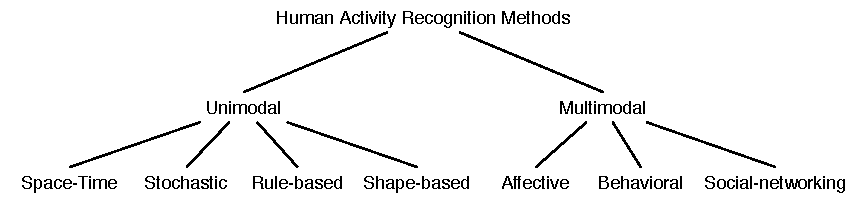
\includegraphics[width=\textwidth,keepaspectratio]
    {images/introduction/har-taxonomy.pdf}
    \caption{Hierarchical categorization of human activity recognition methods}
    \label{har-taxonomy}
\end{figure}

% tendency showing movement in direction of different tests digitized versions



% extend previous research by introducing novel method of drawing pattern analysis 

% Distinction from others
% - luria patterns are rarely used
% - existing studies only analyze whole pattern or strokes
% - logical structure of the pattern is not being taken into account
% - new clustering solution, relatively positioned and sized pattern elements
% - pattern transformation into tree-like graph structures
% - interpretable clusters complimented with parameters
% - anomaly detection 

% Thesis organized as follows
% - 
% - 
% - 


% Main focus of present thesis is to analyze Luria’s drawing patterns of tested individuals, extract interpretable features and produce machine learning model, capable of correct differentiation between groups of healthy controls and Parkinson’s disease patients.

% Luria’s alternating series fine motor tests are being used in psychology and neurology to assess level of disorder in motion planning and execution during handwriting, which is approved biomarker for Parkinson’s disease diagnosis.

% A novel method to analyze Luria’s alternating series patterns drawn during fine motor test constitute main result of the present thesis. Majority of solutions available in the literature are based either on the analysis of entire drawing or individual strokes. Distinctive feature of the proposed approach is that it allows to analyze patterns considering their logical structure with any required level of detail. To achieve this, unique supervised and unsupervised machine learning techniques are applied. Computer vision technique is used to split pattern into logical segments. Based on this information, feature sequences describing different kinematic properties of the drawing are constructed. During next stages, neural-network based models are used to generate feature sequences of the "expected" normal drawing, which allows to highlight "unexpected" regions with anomalies.